\documentclass[11pt,letterpaper,twoside]{book}

% ============================================================================
% PACKAGES
% ============================================================================
\usepackage[utf8]{inputenc}
\usepackage[T1]{fontenc}
\usepackage{lmodern}
\usepackage[margin=1in,inner=1.25in,outer=1in]{geometry}
\usepackage{graphicx}
\usepackage{xcolor}
\usepackage{tikz}
\usepackage{booktabs}
\usepackage{longtable}
\usepackage{array}
\usepackage{tabularx}
\usepackage{multirow}
\usepackage{enumitem}
\usepackage{fancyhdr}
\usepackage{titlesec}
\usepackage{tcolorbox}
\usepackage{amsmath}
\usepackage{amssymb}
\usepackage{hyperref}
\usepackage{cleveref}
\usepackage{siunitx}
\DeclareSIUnit{\sample}{S}
\usepackage{fontawesome5}

% Fix headheight warning from fancyhdr
\setlength{\headheight}{14pt}
\usepackage{caption}
\usepackage{subcaption}
\usepackage{wrapfig}
\usepackage{float}
\usepackage{pdfpages}
\usepackage{microtype}
\usepackage{lipsum}

% ============================================================================
% COLOR DEFINITIONS
% ============================================================================
\definecolor{aoeblue}{RGB}{0,74,127}
\definecolor{aoegold}{RGB}{196,154,0}
\definecolor{darkgreen}{RGB}{0,100,0}
\definecolor{warnorange}{RGB}{230,126,34}
\definecolor{lightblue}{RGB}{230,240,250}
\definecolor{lightgreen}{RGB}{230,250,230}
\definecolor{lightyellow}{RGB}{255,250,230}
\definecolor{lightred}{RGB}{255,235,235}
\definecolor{codegray}{RGB}{245,245,245}

% ============================================================================
% TCOLORBOX CONFIGURATIONS
% ============================================================================
\tcbuselibrary{skins,breakable}

\newtcolorbox{aoeref}{
    colback=lightblue,
    colframe=aoeblue,
    title={\faBook\ AoE Reference},
    fonttitle=\bfseries,
    breakable,
    enhanced,
    left=8pt,
    right=8pt
}

\newtcolorbox{learningobjectives}{
    colback=lightgreen,
    colframe=darkgreen,
    title={\faGraduationCap\ Learning Objectives},
    fonttitle=\bfseries,
    breakable,
    enhanced,
    left=8pt,
    right=8pt
}

\newtcolorbox{projectbox}{
    colback=lightyellow,
    colframe=aoegold,
    title={\faCogs\ Project Description},
    fonttitle=\bfseries,
    breakable,
    enhanced,
    left=8pt,
    right=8pt
}

\newtcolorbox{warningbox}{
    colback=lightred,
    colframe=red!70!black,
    title={\faExclamationTriangle\ Safety Warning},
    fonttitle=\bfseries,
    breakable,
    enhanced,
    left=8pt,
    right=8pt
}

\newtcolorbox{tipbox}{
    colback=codegray,
    colframe=gray!70!black,
    title={\faLightbulb\ Practical Tip},
    fonttitle=\bfseries,
    breakable,
    enhanced,
    left=8pt,
    right=8pt
}

\newtcolorbox{deliverablebox}{
    colback=white,
    colframe=aoeblue,
    title={\faClipboardCheck\ Deliverables},
    fonttitle=\bfseries,
    breakable,
    enhanced,
    left=8pt,
    right=8pt
}

\newtcolorbox{equipmentbox}{
    colback=white,
    colframe=gray!70!black,
    title={\faTools\ Equipment Required},
    fonttitle=\bfseries,
    breakable,
    enhanced,
    left=8pt,
    right=8pt
}

% ============================================================================
% HEADER/FOOTER CONFIGURATION
% ============================================================================
\pagestyle{fancy}
\fancyhf{}
\fancyhead[LE]{\textsl{\leftmark}}
\fancyhead[RO]{\textsl{\rightmark}}
\fancyfoot[LE,RO]{\thepage}
\fancyfoot[C]{\textit{The Art of Electronics Laboratory Curriculum}}
\renewcommand{\headrulewidth}{0.4pt}
\renewcommand{\footrulewidth}{0.4pt}

% ============================================================================
% TITLE FORMATTING
% ============================================================================
\titleformat{\chapter}[display]
    {\normalfont\huge\bfseries\color{aoeblue}}
    {\chaptertitlename\ \thechapter}{20pt}{\Huge}
\titleformat{\section}
    {\normalfont\Large\bfseries\color{aoeblue}}
    {\thesection}{1em}{}
\titleformat{\subsection}
    {\normalfont\large\bfseries\color{aoeblue!80!black}}
    {\thesubsection}{1em}{}
\titleformat{\subsubsection}
    {\normalfont\normalsize\bfseries\color{aoeblue!60!black}}
    {\thesubsubsection}{1em}{}

% ============================================================================
% HYPERREF CONFIGURATION
% ============================================================================
\hypersetup{
    colorlinks=true,
    linkcolor=aoeblue,
    citecolor=darkgreen,
    urlcolor=aoeblue,
    pdftitle={The Art of Electronics Laboratory Curriculum},
    pdfauthor={Electronics Laboratory Course},
    pdfsubject={Project-Based Electronics Curriculum},
    pdfkeywords={electronics, analog, digital, circuits, laboratory}
}

% ============================================================================
% CUSTOM COMMANDS
% ============================================================================
\newcommand{\aoe}{\textit{The Art of Electronics}}
\newcommand{\xchapters}{\textit{The X Chapters}}
\newcommand{\duration}[1]{\textbf{Duration:} #1}
\newcommand{\difficulty}[1]{\textbf{Difficulty:} #1}

% ============================================================================
% DOCUMENT BEGIN
% ============================================================================
\begin{document}

% ============================================================================
% TITLE PAGE
% ============================================================================
\begin{titlepage}
    \centering
    \vspace*{1cm}
    
    \begin{tikzpicture}[remember picture, overlay]
        \fill[aoeblue] (current page.north west) rectangle ([yshift=-4cm]current page.north east);
        \fill[aoegold] ([yshift=-4cm]current page.north west) rectangle ([yshift=-4.3cm]current page.north east);
    \end{tikzpicture}
    
    \vspace{2cm}
    
    {\Huge\bfseries\color{aoeblue} The Art of Electronics\\[0.3cm]}
    {\LARGE\bfseries\color{aoeblue!80!black} Laboratory Curriculum\\[0.5cm]}
    
    \vspace{1cm}
    
    {\Large A Comprehensive Project-Based Course\\[0.3cm]}
    {\large Companion to Horowitz \& Hill's Classic Text\\[0.2cm]}
    {\large with Supplementary Material from \xchapters}
    
    \vspace{2cm}
    
    
\begin{tikzpicture}
        \draw[aoeblue, line width=2pt] (0,0) -- (0,2);
        \draw[aoeblue, line width=2pt] (0,2) -- (1,2);
        \draw[aoegold, line width=2pt] (0,1) -- (0.5,1);
        \draw[aoeblue, line width=2pt] (1.5,0) -- (1.5,2);
        \draw[aoeblue, line width=2pt] (1.5,0) -- (2.5,0);
        \draw[aoeblue, line width=2pt] (1.5,1) -- (2.3,1);
        \draw[aoeblue, line width=2pt] (1.5,2) -- (2.5,2);
        \draw[aoegold, line width=2pt] (3,0) arc[start angle=-90, end angle=90, radius=1];
        \draw[aoeblue, line width=2pt] (3,0) -- (3,2);
        \node[aoeblue] at (1.25,-0.8) {\Large\textbf{AoE}};
    \end{tikzpicture}
    
    \vspace{2cm}
    
    \begin{tcolorbox}[
        colback=lightblue,
        colframe=aoeblue,
        width=0.8\textwidth,
        arc=3mm,
        boxrule=1pt
    ]
    \centering
    \textbf{Course Philosophy:}\\[0.2cm]
    ``Learn by building real instruments you'll keep on your bench.''\\[0.2cm]
    Each phase anchors to specific themes in \aoe{} and culminates in\\
    practical, professional-quality projects.
    \end{tcolorbox}
    
    \vfill
    
    {\large\textbf{Total Duration:} 24--36 weeks (self-paced)}\\[0.3cm]
    {\large\textbf{Prerequisites:} Basic physics, algebra, introductory calculus}\\[0.3cm]
    {\large\textbf{Outcome:} Mixed-signal capstone instrument}
    
    \vspace{1cm}
    
    \begin{tikzpicture}[remember picture, overlay]
        \fill[aoegold] (current page.south west) rectangle ([yshift=0.3cm]current page.south east);
        \fill[aoeblue] ([yshift=0.3cm]current page.south west) rectangle ([yshift=1cm]current page.south east);
    \end{tikzpicture}
    
\end{titlepage}

% ============================================================================
% COPYRIGHT/INFORMATION PAGE
% ============================================================================
\thispagestyle{empty}
\vspace*{\fill}
\begin{center}
\textbf{Course Materials and Licensing}\\[1cm]

This curriculum is designed as a companion to:\\
\textit{The Art of Electronics} (3rd Edition)\\
by Paul Horowitz and Winfield Hill\\
Cambridge University Press, 2015\\[0.5cm]

and\\[0.5cm]

\textit{The Art of Electronics: The X Chapters}\\
by Paul Horowitz and Winfield Hill\\
Cambridge University Press, 2020\\[1cm]

\rule{0.5\textwidth}{0.4pt}\\[1cm]

\textbf{Document Version:} 1.0\\
\textbf{Last Updated:} \today\\[1cm]

\textbf{Recommended Citation:}\\
Electronics Laboratory Curriculum, Project-Based Companion to\\
\textit{The Art of Electronics}, Version 1.0, \the\year.
\end{center}
\vspace*{\fill}
\clearpage

% ============================================================================
% TABLE OF CONTENTS
% ============================================================================
\tableofcontents
\clearpage

% ============================================================================
% PREFACE
% ============================================================================
\chapter*{Preface}
\addcontentsline{toc}{chapter}{Preface}
\markboth{Preface}{Preface}

This curriculum represents a comprehensive, hands-on approach to learning electronics alongside the seminal text \aoe{} by Horowitz and Hill. Rather than treating electronics as a purely theoretical discipline, this course embraces the philosophy that true understanding comes from building, measuring, debugging, and iterating on real circuits.

\section*{Course Philosophy}

The approach taken here differs from traditional electronics courses in several key ways:

\textbf{Project-Centered Learning:} Each phase culminates in one or more substantial projects---not exercises or problem sets, but real instruments and tools you would be proud to keep on your workbench.

\textbf{Iterative Understanding:} You will encounter concepts multiple times at increasing levels of sophistication. A transistor encountered as a simple switch in Phase 1 becomes a precision amplifier stage in Phase 2 and a high-speed buffer in Phase 5.

\textbf{Measurement-Driven Design:} Every design is verified through careful measurement. The difference between calculated and measured performance is not a source of frustration but the most valuable learning opportunity.

\textbf{Integration Over Isolation:} Real instruments are mixed-signal systems combining analog, digital, and power electronics. This curriculum builds toward that integration from the beginning.

\section*{How to Use This Curriculum}

This document can serve multiple purposes:

\begin{itemize}[leftmargin=*]
    \item \textbf{Self-Study Guide:} Work through the phases at your own pace, spending more time on areas that challenge you.
    \item \textbf{Formal Course Spine:} Instructors can use this as a laboratory component for a one-year electronics sequence.
    \item \textbf{Project Reference:} Experienced practitioners can pick individual projects that address specific learning goals.
\end{itemize}

\section*{Prerequisites}

This course assumes:
\begin{itemize}[leftmargin=*]
    \item Basic physics (electricity and magnetism fundamentals)
    \item Algebra and introductory calculus
    \item Willingness to learn circuit simulation software
    \item Access to basic laboratory equipment (detailed in Phase 0)
\end{itemize}

No prior electronics experience is required, though students with some background will progress more quickly through the early phases.

\section*{Acknowledgments}

This curriculum owes its existence to the extraordinary work of Paul Horowitz and Winfield Hill. Their text has educated generations of electronics practitioners, and this course attempts to create a practical companion to their theoretical exposition.

\vspace{1cm}
\hfill\textit{Build well. Measure carefully. Learn continuously.}

\clearpage

% ============================================================================
% PHASE 0: ORIENTATION & LAB SETUP
% ============================================================================
\chapter{Orientation \& Laboratory Setup}
\label{ch:phase0}

\duration{1--2 weeks} \hfill \difficulty{Beginner}

\vspace{0.5cm}

\begin{aoeref}
\textbf{Primary Reading:}
\begin{itemize}[leftmargin=*,nosep]
    \item Preface and Introduction (philosophy of practical electronics)
    \item Appendix A: Oscilloscope Primer
    \item Appendix B: Power Supplies
    \item Appendix N: Laboratory Practice
\end{itemize}

\textbf{Supplementary from \xchapters:}
\begin{itemize}[leftmargin=*,nosep]
    \item Chapter 1x: Real-World Passive Components
\end{itemize}
\end{aoeref}

\vspace{0.5cm}

Before diving into circuit design and construction, you must establish a safe, organized laboratory environment and become comfortable with your measurement tools. This phase, while seemingly administrative, establishes habits that will pay dividends throughout the course.

\section{Phase Overview and Goals}

The primary goal of this phase is to prepare your workspace and establish proficiency with fundamental tools before tackling substantive projects. A well-organized lab with properly understood equipment eliminates countless hours of frustration later.

\begin{learningobjectives}
By the end of this phase, you will be able to:
\begin{enumerate}[leftmargin=*]
    \item Set up a safe, organized electronics workbench with proper ESD protection
    \item Use a digital multimeter (DMM) for voltage, current, and resistance measurements
    \item Operate an oscilloscope including triggering, timebase adjustment, and cursor measurements
    \item Generate and verify test signals using a function generator
    \item Perform basic circuit simulation using SPICE software
    \item Document measurements in a laboratory notebook following professional conventions
    \item Apply AoE's rules-of-thumb to predict and verify circuit behavior
\end{enumerate}
\end{learningobjectives}

\section{Laboratory Setup Requirements}

\subsection{Workbench Organization}

Your workbench is the foundation of all your work. A poorly organized bench leads to mistakes, safety hazards, and wasted time.

\begin{equipmentbox}
\textbf{Essential Workbench Equipment:}
\begin{itemize}[leftmargin=*]
    \item ESD-safe work mat (minimum 24'' $\times$ 36'')
    \item Grounding wrist strap and grounding point
    \item Adequate lighting (adjustable desk lamp with magnification preferred)
    \item Power strip with surge protection (minimum 6 outlets)
    \item Storage bins for components, organized by type
    \item Heat-resistant surface or silicone mat for soldering
    \item Fume extractor or adequate ventilation for soldering
\end{itemize}

\textbf{Essential Hand Tools:}
\begin{itemize}[leftmargin=*]
    \item Diagonal cutters (flush-cut preferred)
    \item Long-nose pliers (smooth and serrated jaws)
    \item Wire strippers (adjustable or multi-gauge)
    \item Precision screwdriver set (Phillips, flathead, Torx)
    \item Tweezers (fine-point, ESD-safe)
    \item Soldering iron (\SI{40}{\watt}--\SI{60}{\watt}, temperature-controlled)
    \item Solder (60/40 or lead-free, 0.031'' diameter)
    \item Solder wick and/or solder sucker for desoldering
    \item Third-hand tool or PCB holder
\end{itemize}
\end{equipmentbox}

\subsection{Test Equipment}

Quality test equipment is essential for meaningful measurements. While professional-grade equipment is ideal, entry-level instruments are sufficient for this course.

\begin{table}[H]
\centering
\caption{Recommended Test Equipment Specifications}
\label{tab:test_equipment}
\begin{tabularx}{\textwidth}{@{}lXX@{}}
\toprule
\textbf{Instrument} & \textbf{Minimum Specifications} & \textbf{Recommended Specifications} \\
\midrule
Digital Multimeter & 3.5 digit, DC/AC voltage and current, resistance, continuity & 4.5 digit, true RMS, capacitance, frequency, temperature \\
\addlinespace
Oscilloscope & 2 channel, \SI{50}{\mega\hertz} bandwidth, \SI{500}{\mega\sample/\second} & 4 channel, \SI{100}{\mega\hertz}+, \SI{1}{\giga\sample/\second}, FFT function \\
\addlinespace
Function Generator & Sine/square/triangle, \SI{1}{\mega\hertz}, amplitude control & DDS-based, \SI{10}{\mega\hertz}+, arbitrary waveform capability \\
\addlinespace
Power Supply & Dual-rail, 0--\SI{30}{\volt}, 0--\SI{3}{\ampere}, current limiting & Triple output, tracking mode, digital display \\
\addlinespace
LCR Meter & Basic capacitance and inductance & Multi-frequency, Q-factor measurement \\
\bottomrule
\end{tabularx}
\end{table}

\subsection{Prototyping Materials}

\begin{itemize}[leftmargin=*]
    \item \textbf{Breadboards:} Minimum 830 tie-points, multiple boards recommended
    \item \textbf{Jumper Wire Kit:} Solid-core 22 AWG in multiple lengths and colors
    \item \textbf{Perfboard/Stripboard:} For semi-permanent prototypes
    \item \textbf{Component Assortments:}
    \begin{itemize}
        \item Resistors: 1/4W, 1\% metal film, E24/E96 series (10$\Omega$ to \SI{1}{\mega\ohm})
        \item Capacitors: Ceramic (10pF to \SI{1}{\micro\farad}), electrolytic (\SI{1}{\micro\farad} to \SI{1000}{\micro\farad})
        \item Diodes: 1N4148 (signal), 1N400x (rectifier), various Zeners
        \item Transistors: 2N3904/2N3906 (BJT), 2N7000/BS170 (MOSFET)
        \item Op-amps: LM358, TL072, OPA2134 (assortment of general-purpose to precision)
        \item Voltage regulators: 78xx/79xx series, LM317
    \end{itemize}
\end{itemize}

\subsection{Software Requirements}

\begin{itemize}[leftmargin=*]
    \item \textbf{SPICE Simulator:} LTspice (free, recommended), ngspice, or TINA-TI
    \item \textbf{Schematic Capture:} KiCad (free, full-featured) or your simulator's built-in editor
    \item \textbf{Documentation:} Laboratory notebook (physical or digital), spreadsheet software
    \item \textbf{Data Analysis:} Python with NumPy/Matplotlib, MATLAB, or similar
\end{itemize}

\section{Safety Fundamentals}

\begin{warningbox}
Electronics work involves electrical hazards, chemical exposure (solder flux, cleaning agents), and burn risks. Always:
\begin{itemize}[leftmargin=*,nosep]
    \item Work on de-energized circuits whenever possible
    \item Use the one-hand rule when measuring live high-voltage circuits
    \item Allow components (especially voltage regulators, power resistors) to cool before handling
    \item Work in a ventilated area when soldering
    \item Wear safety glasses when cutting leads or working with batteries
    \item Never work when fatigued or distracted
\end{itemize}
\end{warningbox}

\subsection{Electrostatic Discharge (ESD) Protection}

ESD can destroy sensitive components (CMOS ICs, MOSFETs, precision op-amps) without any visible damage. Establish these habits:

\begin{enumerate}[leftmargin=*]
    \item Always use a grounded wrist strap when handling sensitive components
    \item Store components in ESD-safe bags or conductive foam
    \item Touch a grounded metal surface before handling components if no wrist strap is available
    \item Use ESD-safe tools (marked with the ESD symbol)
    \item Avoid synthetic clothing and carpeted floors in your work area
\end{enumerate}

\subsection{Power Supply Safety}

\begin{itemize}[leftmargin=*]
    \item Always start with current limiting enabled and set appropriately
    \item Verify power supply polarity before connecting to circuits
    \item Use fuses in permanent installations
    \item Capacitors can retain charge---discharge them before working on circuits
    \item Never exceed component voltage or power ratings
\end{itemize}

\section{Mini-Project 0.1: Lab Power \& Measurement Check}

\begin{projectbox}
\textbf{Project Title:} Linear Voltage Regulator Characterization

\textbf{Objective:} Build a simple linear regulator circuit and use it to practice measurement techniques while verifying AoE's rules-of-thumb about regulator behavior.

\textbf{Time Estimate:} 3--4 hours
\end{projectbox}

\subsection{Background}

Three-terminal voltage regulators (78xx series) are ubiquitous in electronics. Despite their simplicity, they illustrate fundamental concepts: voltage regulation, thermal management, and the trade-offs between linear and switching approaches.

AoE discusses these regulators extensively, providing rules-of-thumb for dropout voltage, ripple rejection, and thermal behavior. This project verifies those predictions experimentally.

\subsection{Circuit Description}

Build a \SI{12}{\volt} to \SI{5}{\volt} linear regulator using a 7805 regulator with proper input and output capacitors.

\begin{figure}[H]
\centering
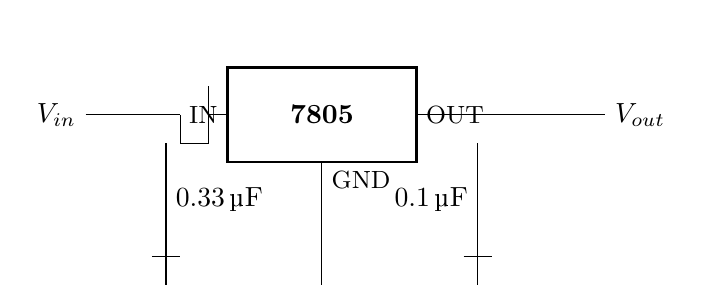
\begin{tikzpicture}[scale=1.2]
    % Input
    \draw (0,0) node[left] {$V_{in}$} -- (1,0);
    \draw (1,0) -- (1,-0.3);
    \draw (1,-0.3) -- (1.3,-0.3);
    \draw (1.3,-0.3) -- (1.3,0.3);
    \draw (1.3,0) -- (1.5,0);
    \draw (0.85,-0.3) -- (0.85,-1.5);
    \node at (0.85,-0.9) [right] {\SI{0.33}{\micro\farad}};
    \draw (0.7,-1.5) -- (1,-1.5);
    \draw (0.85,-1.5) -- (0.85,-1.8);
    \node at (0.85,-1.8) [below] {};
    
    % Regulator
    \draw[thick] (1.5,-0.5) rectangle (3.5,0.5);
    \node at (2.5,0) {\textbf{7805}};
    \draw (1.5,0) node[left] {\small IN};
    \draw (3.5,0) node[right] {\small OUT};
    \draw (2.5,-0.5) -- (2.5,-1);
    \node at (2.5,-0.5) [below right] {\small GND};
    \draw (2.5,-1) -- (2.5,-1.8);
    \node at (2.5,-1.8) [below] {};
    
    % Output
    \draw (3.5,0) -- (4.5,0);
    \draw (4.15,-0.3) -- (4.15,-1.5);
    \node at (4.15,-0.9) [left] {\SI{0.1}{\micro\farad}};
    \draw (4,-1.5) -- (4.3,-1.5);
    \draw (4.15,-1.5) -- (4.15,-1.8);
    \node at (4.15,-1.8) [below] {};
    \draw (4.5,0) -- (5.5,0) node[right] {$V_{out}$};
\end{tikzpicture}
\caption{Basic 7805 linear regulator circuit}
\label{fig:7805_circuit}
\end{figure}

\subsection{Procedure}

\subsubsection{Step 1: Build the Circuit}

\begin{enumerate}[leftmargin=*]
    \item Identify the 7805 pinout (check datasheet---variants exist!)
    \item Install input capacitor (\SI{0.33}{\micro\farad} ceramic) close to the regulator
    \item Install output capacitor (\SI{0.1}{\micro\farad} ceramic) close to the regulator
    \item Add a load resistor (start with \SI{100}{\ohm}, \SI{250}{\milli\watt} dissipation at \SI{5}{\volt})
\end{enumerate}

\subsubsection{Step 2: Line Regulation Measurement}

Line regulation measures output voltage change as input voltage varies.

\begin{enumerate}[leftmargin=*]
    \item Set load to \SI{100}{\ohm} (fixed)
    \item Vary $V_{in}$ from \SI{7}{\volt} to \SI{15}{\volt} in \SI{0.5}{\volt} steps
    \item Record $V_{out}$ at each step
    \item Calculate line regulation: $\frac{\Delta V_{out}}{\Delta V_{in}} \times 100\%$
\end{enumerate}

\subsubsection{Step 3: Load Regulation Measurement}

Load regulation measures output voltage change as load current varies.

\begin{enumerate}[leftmargin=*]
    \item Set $V_{in} = \SI{12}{\volt}$ (fixed)
    \item Vary load from \SI{0}{\milli\ampere} to \SI{500}{\milli\ampere}
    \item Record $V_{out}$ at each load current
    \item Calculate load regulation: $\frac{\Delta V_{out}}{\Delta I_{load}} \times 100\%$
\end{enumerate}

\subsubsection{Step 4: Ripple Rejection Measurement}

\begin{enumerate}[leftmargin=*]
    \item Add a \SI{1}{\volt} peak-to-peak, \SI{120}{\hertz} sine wave to the DC input (simulating rectifier ripple)
    \item Measure input and output ripple with oscilloscope (AC coupling)
    \item Calculate ripple rejection ratio in dB
\end{enumerate}

\subsubsection{Step 5: Thermal Measurement}

\begin{enumerate}[leftmargin=*]
    \item Apply \SI{500}{\milli\ampere} load at $V_{in} = \SI{12}{\volt}$
    \item Calculate power dissipation: $P = (V_{in} - V_{out}) \times I_{load}$
    \item Monitor regulator temperature over 10 minutes
    \item Calculate thermal resistance: $\theta_{JA} = \frac{T_J - T_A}{P}$
\end{enumerate}

\begin{tipbox}
Use a thermocouple or IR thermometer to measure the regulator tab temperature. Be careful---the regulator can get hot enough to cause burns at high power dissipation!
\end{tipbox}

\subsection{Analysis and Comparison with AoE}

After completing measurements, compare your results with the predictions from \aoe:

\begin{table}[H]
\centering
\caption{Comparison of Measured vs. Predicted Performance}
\label{tab:7805_comparison}
\begin{tabularx}{\textwidth}{@{}lXXX@{}}
\toprule
\textbf{Parameter} & \textbf{AoE Typical} & \textbf{Datasheet} & \textbf{Measured} \\
\midrule
Output Voltage & \SI{5.0}{\volt} $\pm$ 4\% & & \\
Line Regulation & \SI{3}{\milli\volt}/V typ. & & \\
Load Regulation & \SI{15}{\milli\volt} typ. & & \\
Ripple Rejection & \SI{70}{\decibel} typ. @120Hz & & \\
Dropout Voltage & \SI{2}{\volt} typ. & & \\
Thermal Resistance & $\sim$\SI{50}{\celsius/\watt} (TO-220) & & \\
\bottomrule
\end{tabularx}
\end{table}

\begin{deliverablebox}
\begin{itemize}[leftmargin=*]
    \item Completed measurement table comparing AoE predictions to actual results
    \item Line regulation plot ($V_{out}$ vs $V_{in}$)
    \item Load regulation plot ($V_{out}$ vs $I_{load}$)
    \item Oscilloscope screenshot showing input and output ripple
    \item Thermal measurement data and calculation
    \item Written analysis: ``What I expected vs. what I measured, and why they might differ''
\end{itemize}
\end{deliverablebox}

\section{Mini-Project 0.2: Signal Visualization Workshop}

\begin{projectbox}
\textbf{Project Title:} Oscilloscope and Function Generator Proficiency

\textbf{Objective:} Develop fluency with oscilloscope operation through systematic exploration of waveform generation, measurement, and documentation.

\textbf{Time Estimate:} 2--3 hours
\end{projectbox}

\subsection{Exercises}

\subsubsection{Exercise A: Basic Waveform Generation and Measurement}

\begin{enumerate}[leftmargin=*]
    \item Generate a \SI{1}{\kilo\hertz} sine wave, \SI{2}{\volt} peak-to-peak
    \item Display on oscilloscope with proper scaling
    \item Measure and record: frequency, period, peak-to-peak amplitude, RMS amplitude
    \item Repeat for square and triangle waves at the same frequency
\end{enumerate}

\subsubsection{Exercise B: Triggering Mastery}

\begin{enumerate}[leftmargin=*]
    \item Generate a pulse train (variable duty cycle)
    \item Practice triggering: rising edge, falling edge, level adjustment
    \item Generate a complex waveform (AM modulated or burst mode)
    \item Achieve stable triggering on the modulation envelope
\end{enumerate}

\subsubsection{Exercise C: Rise Time and Bandwidth}

\begin{enumerate}[leftmargin=*]
    \item Generate a fast square wave (\SI{1}{\mega\hertz} or higher)
    \item Measure rise time using oscilloscope cursors
    \item Calculate the approximate bandwidth of your signal source
    \item Understand the relationship: $BW \approx \frac{0.35}{t_r}$
\end{enumerate}

\subsubsection{Exercise D: SPICE Simulation Correlation}

\begin{enumerate}[leftmargin=*]
    \item Simulate a simple RC low-pass filter in SPICE
    \item Build the same filter on breadboard
    \item Apply a square wave input and compare:
    \begin{itemize}
        \item Simulated output waveform
        \item Measured output waveform
    \end{itemize}
    \item Document any differences and hypothesize causes
\end{enumerate}

\begin{deliverablebox}
\begin{itemize}[leftmargin=*]
    \item Annotated oscilloscope screenshots for each waveform type
    \item Rise time measurement with calculation showing bandwidth
    \item SPICE simulation output and corresponding oscilloscope capture
    \item Brief written comparison of simulation vs. measurement
\end{itemize}
\end{deliverablebox}

\section{Laboratory Notebook Best Practices}

Throughout this course, maintain a laboratory notebook documenting all work. Good documentation habits are essential for:

\begin{itemize}[leftmargin=*]
    \item Debugging circuits that ``worked yesterday''
    \item Building on previous work without re-learning
    \item Professional engineering practice
\end{itemize}

\subsection{Notebook Format}

Each entry should include:

\begin{enumerate}[leftmargin=*]
    \item \textbf{Date and Title:} Clear identification of the work session
    \item \textbf{Objective:} What you intend to accomplish
    \item \textbf{Schematic:} Hand-drawn or printed, with component values
    \item \textbf{Procedure:} Steps taken, in enough detail to reproduce
    \item \textbf{Data:} Raw measurements in tables or plots
    \item \textbf{Observations:} Unexpected behavior, anomalies, questions
    \item \textbf{Conclusions:} What worked, what didn't, next steps
\end{enumerate}

\begin{tipbox}
Photograph your breadboard layouts and paste them into your notebook. When debugging later, you'll appreciate having a record of exactly how things were connected.
\end{tipbox}

\section{Phase 0 Checklist}

Before proceeding to Phase 1, verify:

\begin{itemize}
    \item[$\square$] Laboratory workspace is organized with proper ESD protection
    \item[$\square$] All test equipment is functional and calibrated
    \item[$\square$] SPICE software is installed and you can run a simple simulation
    \item[$\square$] Mini-Project 0.1 (regulator characterization) completed with documentation
    \item[$\square$] Mini-Project 0.2 (oscilloscope proficiency) completed with documentation
    \item[$\square$] Laboratory notebook established with consistent formatting
\end{itemize}

\clearpage

% ============================================================================
% PHASE 1: ANALOG FOUNDATIONS
% ============================================================================
\chapter{Analog Foundations \& Building Blocks}
\label{ch:phase1}

\duration{3--4 weeks} \hfill \difficulty{Beginner to Intermediate}

\vspace{0.5cm}

\begin{aoeref}
\textbf{Primary Reading:}
\begin{itemize}[leftmargin=*,nosep]
    \item Chapter 1: Foundations (1.1--1.7)
    \item Chapter 2: Bipolar Transistors (2.1--2.3)
    \item Chapter 3: Field-Effect Transistors (3.1--3.2)
    \item Chapter 4: Operational Amplifiers (4.1--4.4)
    \item Chapter 6: Filters (6.1--6.2)
\end{itemize}

\textbf{Supplementary from \xchapters:}
\begin{itemize}[leftmargin=*,nosep]
    \item Chapter 4x: Advanced Topics in Op-Amps
\end{itemize}
\end{aoeref}

\vspace{0.5cm}

This phase establishes the analog foundation upon which all subsequent work builds. You will design, build, and characterize the fundamental building blocks that appear in virtually every analog system: amplifiers, buffers, filters, and switches.

\section{Phase Overview and Goals}

The goal of this phase is to develop intuition for analog circuit behavior through hands-on construction and measurement. By the end of this phase, you should be able to look at a new analog circuit and predict its approximate behavior before simulation or measurement.

\begin{learningobjectives}
By the end of this phase, you will be able to:
\begin{enumerate}[leftmargin=*]
    \item Design and analyze inverting, non-inverting, and buffer op-amp configurations
    \item Calculate gain, bandwidth, input impedance, and output impedance for basic amplifier stages
    \item Design active low-pass and high-pass filters with specified cutoff frequencies
    \item Configure transistors as switches for driving LEDs, relays, and other loads
    \item Implement emitter/source followers as buffers and understand their loading effects
    \item Use SPICE simulation to predict circuit behavior and compare with measurements
    \item Recognize and diagnose common problems: oscillation, clipping, loading, offset
\end{enumerate}
\end{learningobjectives}

\section{Theoretical Foundation}

\subsection{The Op-Amp as a Universal Building Block}

The operational amplifier is perhaps the most versatile component in analog design. Understanding its behavior under negative feedback is essential.

\subsubsection{Golden Rules of Op-Amp Analysis}

When an op-amp operates with negative feedback:

\begin{enumerate}[leftmargin=*]
    \item \textbf{The output adjusts to make the voltage difference between the inputs zero.}
    
    $V_+ \approx V_-$ (virtual short)
    
    \item \textbf{The inputs draw no current.}
    
    $I_+ \approx I_- \approx 0$ (for most practical purposes)
\end{enumerate}

These ``golden rules'' enable quick analysis of most op-amp circuits.

\subsubsection{Gain-Bandwidth Product}

Real op-amps have finite gain that rolls off with frequency. The gain-bandwidth product (GBW or GBP) is approximately constant:

\begin{equation}
    GBW = A_{OL} \times f_{OL} = A_{CL} \times f_{CL}
\end{equation}

where $A_{OL}$ is open-loop gain, $f_{OL}$ is open-loop bandwidth, $A_{CL}$ is closed-loop gain, and $f_{CL}$ is closed-loop bandwidth.

\begin{tipbox}
An op-amp with \SI{1}{\mega\hertz} GBW configured for gain of 10 will have a bandwidth of approximately \SI{100}{\kilo\hertz}. This trade-off between gain and bandwidth is fundamental.
\end{tipbox}

\subsection{Transistor Fundamentals}

\subsubsection{BJT as a Switch}

For switching applications, operate the transistor in saturation (fully on) or cutoff (fully off):

\begin{itemize}[leftmargin=*]
    \item \textbf{Cutoff:} $V_{BE} < \SI{0.6}{\volt}$ --- transistor is off, $I_C \approx 0$
    \item \textbf{Saturation:} $I_B > \frac{I_C}{\beta_{forced}}$ --- transistor is fully on, $V_{CE(sat)} \approx \SI{0.1}{\volt}$--$\SI{0.3}{\volt}$
\end{itemize}

The base resistor is chosen to ensure saturation with margin:

\begin{equation}
    R_B = \frac{V_{drive} - V_{BE}}{I_B} = \frac{V_{drive} - V_{BE}}{\frac{I_C}{\beta / 10}}
\end{equation}

where the factor of 10 ensures hard saturation.

\subsubsection{Emitter Follower (Common Collector)}

The emitter follower provides:
\begin{itemize}[leftmargin=*]
    \item Voltage gain $\approx 1$ (unity)
    \item High input impedance ($\approx \beta \times R_E$)
    \item Low output impedance ($\approx R_S / \beta$)
\end{itemize}

This makes it ideal as a buffer between high-impedance sources and low-impedance loads.

\subsection{Filter Fundamentals}

\subsubsection{First-Order Filters}

A first-order filter has a single pole and provides \SI{20}{\decibel}/decade (or \SI{6}{\decibel}/octave) rolloff.

\textbf{Low-pass RC filter:}
\begin{equation}
    f_c = \frac{1}{2\pi RC}
\end{equation}

\textbf{High-pass RC filter:} Same equation, but the capacitor and resistor positions are swapped.

\subsubsection{Second-Order Active Filters}

Active filters using op-amps can provide:
\begin{itemize}[leftmargin=*]
    \item Steeper rolloff (\SI{40}{\decibel}/decade for second-order)
    \item Controlled damping (Q factor)
    \item Gain in the passband
    \item High input impedance
\end{itemize}

The Sallen-Key topology is the most common for second-order filters.

\section{Core Project: Analog Building-Block Toolkit Board}

\begin{projectbox}
\textbf{Project Title:} Modular Analog Toolkit

\textbf{Objective:} Create a collection of characterized analog building blocks that can be reconfigured for various applications. This board becomes your ``analog Lego set'' for future projects.

\textbf{Time Estimate:} 8--12 hours (design, build, characterize)
\end{projectbox}

\subsection{System Requirements}

Your toolkit board should include the following subsystems:

\begin{table}[H]
\centering
\caption{Analog Toolkit Subsystem Requirements}
\label{tab:toolkit_requirements}
\begin{tabularx}{\textwidth}{@{}lXl@{}}
\toprule
\textbf{Subsystem} & \textbf{Specifications} & \textbf{Quantity} \\
\midrule
General-Purpose Op-Amp Stage & Configurable as inverting, non-inverting, or buffer; selectable gain (1, 10, 100); bandwidth $>$ \SI{100}{\kilo\hertz} at unity gain & 2 \\
\addlinespace
Active Low-Pass Filter & Second-order Sallen-Key; $f_c$ selectable (\SI{1}{\kilo\hertz} or \SI{10}{\kilo\hertz}); Butterworth response & 1 \\
\addlinespace
Active High-Pass Filter & Second-order Sallen-Key; $f_c$ = \SI{100}{\hertz}; Butterworth response & 1 \\
\addlinespace
Transistor Switch & NPN, capable of \SI{500}{\milli\ampere}; LED indicator; flyback protection for inductive loads & 1 \\
\addlinespace
Emitter Follower Buffer & Input impedance $>$ \SI{100}{\kilo\ohm}; output capable of driving \SI{50}{\ohm} & 1 \\
\bottomrule
\end{tabularx}
\end{table}

\subsection{Subsystem 1: Configurable Op-Amp Stage}

\subsubsection{Design}

Use a quality general-purpose op-amp such as the TL072 or OPA2134. The configuration should be selectable via jumpers.

\begin{figure}[H]
\centering
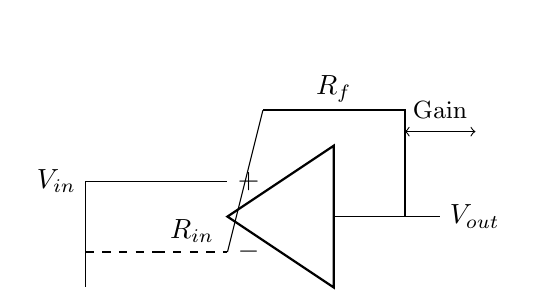
\begin{tikzpicture}[scale=0.9]
    % Op-amp symbol
    \draw[thick] (2,0) -- (3.5,1) -- (3.5,-1) -- cycle;
    \draw (2.3,0.5) node {$+$};
    \draw (2.3,-0.5) node {$-$};
    
    % Input
    \draw (0,0.5) node[left] {$V_{in}$} -- (2,0.5);
    
    % Feedback resistor
    \draw (3.5,0) -- (4.5,0);
    \draw[thick] (4.5,0) -- (4.5,1.5) -- (2.5,1.5);
    \draw (2.5,1.5) -- (2,-0.5);
    \node at (3.5,1.8) {$R_f$};
    
    % Input resistor (for inverting)
    \draw[dashed] (0,-0.5) -- (1,-0.5);
    \draw[thick,dashed] (1,-0.5) -- (2,-0.5);
    \node at (1.5,-0.2) {$R_{in}$};
    
    % Output
    \draw (3.5,0) -- (5,0) node[right] {$V_{out}$};
    
    % Ground reference
    \draw (0,0.5) -- (0,-1);
    \node at (0,-1) [below] {};
    
    % Jumper indicators
    \draw[<->] (4.5,1.2) -- (5.5,1.2);
    \node at (5,1.5) {\small Gain};
\end{tikzpicture}
\caption{Configurable op-amp stage concept (simplified)}
\label{fig:opamp_config}
\end{figure}

\textbf{Gain settings} should be implemented using precision resistor networks and DIP switches or jumpers:

\begin{itemize}[leftmargin=*]
    \item Unity gain (buffer): $R_f = 0$, $R_{in} = \infty$
    \item Gain of 10: $R_f = \SI{10}{\kilo\ohm}$, $R_{in} = \SI{1}{\kilo\ohm}$ (inverting)
    \item Gain of 100: $R_f = \SI{100}{\kilo\ohm}$, $R_{in} = \SI{1}{\kilo\ohm}$ (inverting)
\end{itemize}

\subsubsection{Characterization Requirements}

For each gain setting, measure and document:

\begin{enumerate}[leftmargin=*]
    \item DC gain (apply DC input, measure DC output)
    \item -3 dB bandwidth (frequency at which gain drops by 3 dB)
    \item Input offset voltage
    \item Output swing limits (at the load you'll typically use)
    \item Slew rate (using square wave input)
\end{enumerate}

\subsection{Subsystem 2: Second-Order Active Low-Pass Filter}

\subsubsection{Design}

Implement a Sallen-Key low-pass filter with Butterworth response (Q = 0.707).

For a Sallen-Key low-pass filter with equal resistors ($R_1 = R_2 = R$) and a damping factor for Butterworth response:

\begin{equation}
    f_c = \frac{1}{2\pi R\sqrt{C_1 C_2}}
\end{equation}

For Butterworth response with unity gain: $C_2 = 2C_1$.

\textbf{Design example for $f_c = \SI{1}{\kilo\hertz}$:}

Choose $R = \SI{10}{\kilo\ohm}$, then:
\begin{align}
    C_1 &= \frac{1}{2\pi \times 10^4 \times 10^3 \times \sqrt{2}} \approx \SI{11.2}{\nano\farad} \\
    C_2 &= 2 C_1 \approx \SI{22.4}{\nano\farad}
\end{align}

Use standard values: $C_1 = \SI{10}{\nano\farad}$, $C_2 = \SI{22}{\nano\farad}$.

\subsubsection{Characterization Requirements}

\begin{enumerate}[leftmargin=*]
    \item Measure frequency response from \SI{10}{\hertz} to \SI{100}{\kilo\hertz}
    \item Plot Bode diagram (magnitude and phase)
    \item Verify -3 dB point matches design
    \item Verify rolloff rate (\SI{40}{\decibel}/decade beyond $f_c$)
    \item Check for any peaking near $f_c$ (indicates Q too high)
\end{enumerate}

\subsection{Subsystem 3: Transistor Switch}

\subsubsection{Design}

Use a general-purpose NPN transistor (2N3904 or 2N2222) to switch loads up to \SI{500}{\milli\ampere}.

\textbf{Key design considerations:}

\begin{itemize}[leftmargin=*]
    \item Calculate base resistor for hard saturation at maximum load
    \item Include flyback diode (1N4148) for inductive loads
    \item Add LED indicator to show switch state
\end{itemize}

\textbf{Base resistor calculation:}

For $I_C = \SI{500}{\milli\ampere}$, $\beta_{min} = 50$, and a forced $\beta$ of 10 for hard saturation:

\begin{equation}
    I_B = \frac{I_C}{10} = \SI{50}{\milli\ampere}
\end{equation}

For a \SI{5}{\volt} drive signal:
\begin{equation}
    R_B = \frac{V_{drive} - V_{BE}}{I_B} = \frac{5 - 0.7}{0.05} = \SI{86}{\ohm}
\end{equation}

Use $R_B = \SI{82}{\ohm}$ (standard value).

\subsubsection{Characterization Requirements}

\begin{enumerate}[leftmargin=*]
    \item Measure $V_{CE(sat)}$ at various collector currents
    \item Measure switching speed (rise and fall times)
    \item Verify proper operation with inductive load (observe flyback diode clamping)
    \item Measure power dissipation and temperature rise at maximum current
\end{enumerate}

\subsection{Subsystem 4: Emitter Follower Buffer}

\subsubsection{Design}

The emitter follower provides current gain while maintaining approximately unity voltage gain.

\textbf{Key specifications:}
\begin{itemize}[leftmargin=*]
    \item Input impedance $>$ \SI{100}{\kilo\ohm}
    \item Output impedance $<$ \SI{100}{\ohm}
    \item Capable of driving \SI{50}{\ohm} loads
\end{itemize}

For high input impedance, consider using a Darlington pair or a JFET input stage.

\subsubsection{Characterization Requirements}

\begin{enumerate}[leftmargin=*]
    \item Measure voltage gain at various frequencies
    \item Measure input impedance using the voltage divider method
    \item Measure output impedance by loading with known resistors
    \item Observe distortion (crossover, clipping) at various output levels
\end{enumerate}

\subsection{System Integration}

Once individual subsystems are characterized, connect them in series to verify proper operation:

\begin{enumerate}[leftmargin=*]
    \item Signal source $\rightarrow$ Buffer $\rightarrow$ Low-pass filter $\rightarrow$ Amplifier $\rightarrow$ Load
    \item Verify that loading effects match predictions
    \item Document the overall frequency response
\end{enumerate}

\begin{deliverablebox}
\textbf{Phase 1 Deliverables:}
\begin{itemize}[leftmargin=*]
    \item Complete schematic of toolkit board with component values and AoE references
    \item SPICE simulation files for each subsystem
    \item Measured Bode plots for filter and amplifier stages
    \item Comparison table: ``Simulated vs. Measured Performance''
    \item Photographs of completed board with labeled subsystems
    \item Written reflection: ``What I predicted vs. what I observed, and lessons learned''
\end{itemize}
\end{deliverablebox}

\section{Troubleshooting Guide}

\subsection{Op-Amp Circuits}

\begin{table}[H]
\centering
\caption{Common Op-Amp Problems and Solutions}
\label{tab:opamp_troubleshooting}
\begin{tabularx}{\textwidth}{@{}lXX@{}}
\toprule
\textbf{Symptom} & \textbf{Likely Cause} & \textbf{Solution} \\
\midrule
Output stuck at rail & Open feedback path or positive feedback & Check feedback resistor connections; verify inverting input \\
\addlinespace
Oscillation at high frequency & Insufficient phase margin & Add compensation capacitor; reduce gain at high frequencies \\
\addlinespace
Large DC offset at output & Input offset voltage amplified by gain & Use precision op-amp; add offset trim circuit \\
\addlinespace
Distorted output & Output hitting rail; slew rate limiting & Reduce input amplitude; use faster op-amp \\
\addlinespace
Reduced bandwidth & Op-amp not specified for high frequency & Check GBW; use appropriate op-amp for application \\
\bottomrule
\end{tabularx}
\end{table}

\subsection{Transistor Circuits}

\begin{table}[H]
\centering
\caption{Common Transistor Problems and Solutions}
\label{tab:transistor_troubleshooting}
\begin{tabularx}{\textwidth}{@{}lXX@{}}
\toprule
\textbf{Symptom} & \textbf{Likely Cause} & \textbf{Solution} \\
\midrule
Transistor always off & Insufficient base current; wrong polarity & Check base resistor value; verify NPN vs. PNP \\
\addlinespace
Transistor always on & Base resistor too small; collector-emitter short & Increase base resistor; replace transistor \\
\addlinespace
High $V_{CE}$ when ``on'' & Not fully saturated & Decrease base resistor to increase $I_B$ \\
\addlinespace
Transistor overheating & Operating in linear region or overcurrent & Ensure hard saturation; verify load current \\
\addlinespace
Voltage spikes at turnoff & Inductive load kickback & Add flyback diode across load \\
\bottomrule
\end{tabularx}
\end{table}

\section{Phase 1 Checklist}

Before proceeding to Phase 2, verify:

\begin{itemize}
    \item[$\square$] All toolkit subsystems are built and functional
    \item[$\square$] Characterization data collected for each subsystem
    \item[$\square$] SPICE simulations completed and compared with measurements
    \item[$\square$] Bode plots generated for filter and amplifier stages
    \item[$\square$] Documentation complete with schematics and photographs
    \item[$\square$] AoE sections read and rules-of-thumb verified experimentally
\end{itemize}

\clearpage

% ============================================================================
% PHASE 2: PRECISION & LOW-NOISE INSTRUMENTATION
% ============================================================================
\chapter{Precision \& Low-Noise Instrumentation}
\label{ch:phase2}

\duration{4--5 weeks} \hfill \difficulty{Intermediate}

\vspace{0.5cm}

\begin{aoeref}
\textbf{Primary Reading:}
\begin{itemize}[leftmargin=*,nosep]
    \item Chapter 5: Precision Circuits (5.1--5.12)
    \item Chapter 8: Low-Noise Techniques (8.1--8.11)
    \item Chapter 4: Op-Amps IV (4.5--4.6, Instrumentation Amplifiers)
\end{itemize}

\textbf{Supplementary from \xchapters:}
\begin{itemize}[leftmargin=*,nosep]
    \item Chapter 5x: Precision Techniques Expanded
    \item Chapter 8x: Noise in Depth
\end{itemize}
\end{aoeref}

\vspace{0.5cm}

This phase transitions from ``making circuits work'' to ``making circuits work precisely and quietly.'' You will learn to deal with microvolt-level signals, understand noise sources, and apply techniques that distinguish professional instrumentation from hobbyist projects.

\section{Phase Overview and Goals}

Precision instrumentation is where electronics becomes truly challenging---and rewarding. A circuit that functions perfectly at the millivolt level may fail catastrophically when you need microvolt resolution. Understanding and controlling noise, offset, drift, and grounding are essential skills.

\begin{learningobjectives}
By the end of this phase, you will be able to:
\begin{enumerate}[leftmargin=*]
    \item Design instrumentation amplifiers for differential measurements
    \item Design transimpedance amplifiers for photodiode and other current-output sensors
    \item Calculate noise budgets including thermal, shot, and 1/f noise contributions
    \item Apply proper grounding, shielding, and layout techniques for low-noise circuits
    \item Select precision references and understand their specifications
    \item Implement signal conditioning chains with defined accuracy and resolution
    \item Debug noise problems systematically using spectral analysis
\end{enumerate}
\end{learningobjectives}

\section{Noise Fundamentals}

\subsection{Types of Noise}

Understanding noise sources is essential for low-noise design:

\subsubsection{Thermal Noise (Johnson-Nyquist Noise)}

Every resistor generates noise due to thermal agitation of electrons:

\begin{equation}
    e_n = \sqrt{4 k_B T R \Delta f}
\end{equation}

where $k_B = \SI{1.38e-23}{\joule/\kelvin}$, $T$ is absolute temperature (K), $R$ is resistance ($\Omega$), and $\Delta f$ is bandwidth (Hz).

At room temperature (\SI{300}{\kelvin}):
\begin{equation}
    e_n \approx \SI{4}{\nano\volt/\sqrt{\hertz}} \times \sqrt{R_{k\Omega}}
\end{equation}

\textbf{Example:} A \SI{10}{\kilo\ohm} resistor has approximately $\SI{4}{\nano\volt/\sqrt{\hertz}} \times \sqrt{10} \approx \SI{12.6}{\nano\volt/\sqrt{\hertz}}$.

\subsubsection{Shot Noise}

Current flowing through a junction exhibits shot noise:

\begin{equation}
    i_n = \sqrt{2 q I \Delta f}
\end{equation}

where $q = \SI{1.6e-19}{\coulomb}$ is the electron charge and $I$ is DC current.

\subsubsection{1/f Noise (Flicker Noise)}

Noise that increases at low frequencies, typically specified as noise density at some reference frequency (often \SI{1}{\hertz} or \SI{10}{\hertz}).

\subsection{Noise Calculations}

When combining multiple noise sources, they add in quadrature (RMS sum):

\begin{equation}
    e_{total} = \sqrt{e_1^2 + e_2^2 + e_3^2 + \ldots}
\end{equation}

\begin{tipbox}
A source contributing less than 1/3 of the dominant noise source adds less than 5\% to the total noise. Focus your efforts on the largest contributors.
\end{tipbox}

\section{Precision Amplifier Topologies}

\subsection{The Instrumentation Amplifier}

The instrumentation amplifier (in-amp) provides:
\begin{itemize}[leftmargin=*]
    \item Very high input impedance on both inputs
    \item High common-mode rejection ratio (CMRR)
    \item Gain set by a single resistor
    \item Low drift and offset
\end{itemize}

The classic three-op-amp instrumentation amplifier uses a differential amplifier preceded by two non-inverting buffers with shared feedback.

\textbf{Gain equation:}
\begin{equation}
    G = \left(1 + \frac{2R_1}{R_G}\right) \times \frac{R_3}{R_2}
\end{equation}

For matched resistors and the standard configuration:
\begin{equation}
    G = 1 + \frac{2R}{R_G}
\end{equation}

\subsection{The Transimpedance Amplifier (TIA)}

For current-output sensors (photodiodes, PMTs), the transimpedance amplifier converts current to voltage:

\begin{equation}
    V_{out} = -I_{in} \times R_f
\end{equation}

\textbf{Key design considerations:}
\begin{itemize}[leftmargin=*]
    \item Feedback capacitor ($C_f$) for stability (sensor capacitance causes phase shift)
    \item Op-amp input bias current adds to sensor current
    \item Op-amp current noise appears at output multiplied by feedback resistance
\end{itemize}

The feedback capacitor should satisfy:
\begin{equation}
    C_f \geq \sqrt{\frac{C_{in}}{2\pi R_f GBW}}
\end{equation}

where $C_{in}$ is the total input capacitance and $GBW$ is the op-amp gain-bandwidth product.

\section{Core Project: Sensor Front-End \& Data Logger}

\begin{projectbox}
\textbf{Project Title:} Precision Sensor Acquisition System

\textbf{Objective:} Design and build a complete signal chain from sensor to digital output, applying precision techniques to achieve a defined accuracy and resolution.

\textbf{Sensor Options:}
\begin{itemize}[leftmargin=*]
    \item \textbf{Option A:} Photodiode light meter (transimpedance amplifier approach)
    \item \textbf{Option B:} Strain gauge / load cell (instrumentation amplifier approach)
    \item \textbf{Option C:} Thermocouple / RTD (precision low-level measurement)
\end{itemize}

\textbf{Time Estimate:} 15--20 hours
\end{projectbox}

\subsection{System Architecture}

Regardless of sensor choice, your system should include:

\begin{enumerate}[leftmargin=*]
    \item \textbf{Sensor Interface:} Appropriate front-end for your sensor type
    \item \textbf{Analog Signal Conditioning:} Amplification, filtering, level shifting as needed
    \item \textbf{Voltage Reference:} Stable reference for ratiometric measurement or ADC reference
    \item \textbf{Analog-to-Digital Conversion:} Resolution appropriate to measurement needs
    \item \textbf{Data Logging:} Serial output or SD card storage
\end{enumerate}

\subsection{Option A: Photodiode Light Meter}

\subsubsection{Specifications}

\begin{table}[H]
\centering
\caption{Photodiode Light Meter Specifications}
\label{tab:photodiode_specs}
\begin{tabularx}{\textwidth}{@{}lX@{}}
\toprule
\textbf{Parameter} & \textbf{Target Value} \\
\midrule
Measurement Range & \SI{1}{\nano\ampere} to \SI{1}{\milli\ampere} (6 decades) \\
Resolution & 12 bits within each range \\
Bandwidth & DC to \SI{100}{\hertz} \\
Noise Floor & $<$ \SI{1}{\pico\ampere} RMS in low-current range \\
\bottomrule
\end{tabularx}
\end{table}

\subsubsection{Design Approach}

\begin{enumerate}[leftmargin=*]
    \item \textbf{TIA Stage:} Use a low-bias-current op-amp (FET input) with switchable feedback resistors for range selection
    \item \textbf{Gain Stage:} Additional amplification to fill ADC input range
    \item \textbf{Anti-Alias Filter:} Low-pass filter with $f_c \approx \SI{100}{\hertz}$
    \item \textbf{ADC:} 16-bit sigma-delta ADC for best low-frequency resolution
\end{enumerate}

\textbf{Noise Budget Example:}

For the lowest range (highest sensitivity), with $R_f = \SI{10}{\mega\ohm}$:

\begin{align}
    e_n(R_f) &= \SI{4}{\nano\volt/\sqrt{\hertz}} \times \sqrt{10000} = \SI{400}{\nano\volt/\sqrt{\hertz}} \\
    \text{In \SI{100}{\hertz} BW:} \quad e_n &= 400 \times \sqrt{100} = \SI{4}{\micro\volt} \\
    \text{Referred to input:} \quad i_n &= \frac{\SI{4}{\micro\volt}}{\SI{10}{\mega\ohm}} = \SI{0.4}{\pico\ampere}
\end{align}

This meets the \SI{1}{\pico\ampere} noise floor target.

\subsection{Option B: Strain Gauge / Load Cell}

\subsubsection{Specifications}

\begin{table}[H]
\centering
\caption{Load Cell Measurement Specifications}
\label{tab:loadcell_specs}
\begin{tabularx}{\textwidth}{@{}lX@{}}
\toprule
\textbf{Parameter} & \textbf{Target Value} \\
\midrule
Full-Scale Input & \SI{10}{\milli\volt} (typical load cell output at full load) \\
Resolution & 1 part in 10,000 (approximately 14 bits) \\
Accuracy & $\pm$0.1\% of full scale after calibration \\
CMRR & $>$ \SI{100}{\decibel} \\
Bandwidth & DC to \SI{10}{\hertz} \\
\bottomrule
\end{tabularx}
\end{table}

\subsubsection{Design Approach}

\begin{enumerate}[leftmargin=*]
    \item \textbf{Bridge Excitation:} Stable voltage reference for bridge excitation
    \item \textbf{Instrumentation Amplifier:} High-CMRR in-amp (INA128, AD620, or similar)
    \item \textbf{Gain Calculation:} For \SI{10}{\milli\volt} input to \SI{2.5}{\volt} output: $G = 250$
    \item \textbf{ADC:} 16-bit or 24-bit ADC with differential input
\end{enumerate}

\subsection{Option C: Thermocouple / RTD}

\subsubsection{Design Approach}

For thermocouples:
\begin{itemize}[leftmargin=*]
    \item Signal level: \SI{40}{\micro\volt/\celsius} (Type K)
    \item Cold junction compensation required
    \item Typically use integrated solutions (MAX31855, AD849x) or precision front-ends
\end{itemize}

For RTDs:
\begin{itemize}[leftmargin=*]
    \item Resistance measurement with minimal self-heating
    \item 3-wire or 4-wire configuration for lead resistance cancellation
    \item Current source excitation with precision measurement
\end{itemize}

\subsection{Noise Budget Template}

Complete this table for your chosen sensor:

\begin{table}[H]
\centering
\caption{Noise Budget Template}
\label{tab:noise_budget}
\begin{tabularx}{\textwidth}{@{}lXXX@{}}
\toprule
\textbf{Noise Source} & \textbf{Spectral Density} & \textbf{Equivalent BW} & \textbf{RMS Contribution} \\
\midrule
Op-amp voltage noise & \si{\nano\volt/\sqrt{\hertz}} & \si{\hertz} & \si{\nano\volt} \\
Op-amp current noise & \si{\pico\ampere/\sqrt{\hertz}} & \si{\hertz} & \si{\pico\ampere} \\
Feedback resistor thermal & \si{\nano\volt/\sqrt{\hertz}} & \si{\hertz} & \si{\nano\volt} \\
Source resistance thermal & \si{\nano\volt/\sqrt{\hertz}} & \si{\hertz} & \si{\nano\volt} \\
ADC quantization & --- & --- & \si{LSB} \\
\midrule
\textbf{Total (RSS)} & --- & --- & \textbf{---} \\
\bottomrule
\end{tabularx}
\end{table}

\subsection{Grounding and Shielding Practices}

\begin{warningbox}
Ground loops are the most common source of problems in precision instrumentation. Follow these rules religiously:
\begin{itemize}[leftmargin=*,nosep]
    \item Use star grounding---all ground returns meet at a single point
    \item Keep signal ground and power ground separate until the star point
    \item Shield cables and connect the shield at one end only
    \item Use differential measurements whenever possible
    \item Route sensitive signals away from high-current or switching circuits
\end{itemize}
\end{warningbox}

\begin{deliverablebox}
\textbf{Phase 2 Deliverables:}
\begin{itemize}[leftmargin=*]
    \item System block diagram showing all analog and digital subsystems
    \item Complete noise budget spreadsheet with calculated and measured values
    \item Schematic with detailed grounding and shielding notes
    \item Calibration data: measured vs. known stimulus at multiple points
    \item Noise floor measurement: output with input shorted/terminated
    \item Time-series data log demonstrating successful measurement
    \item Written analysis: ``Where the noise came from and how I reduced it''
\end{itemize}
\end{deliverablebox}

\section{Phase 2 Checklist}

Before proceeding to Phase 3, verify:

\begin{itemize}
    \item[$\square$] Complete signal chain designed and simulated
    \item[$\square$] Noise budget calculated with all significant contributors
    \item[$\square$] Circuit built with proper grounding and shielding
    \item[$\square$] Noise floor measured and compared with budget
    \item[$\square$] System calibrated against known reference
    \item[$\square$] Data logging functional and producing meaningful output
    \item[$\square$] Documentation complete with noise analysis and calibration data
\end{itemize}

\clearpage

% ============================================================================
% PHASE 3: POWER ELECTRONICS & PROTECTION
% ============================================================================
\chapter{Power Electronics \& Protection}
\label{ch:phase3}

\duration{4--5 weeks} \hfill \difficulty{Intermediate to Advanced}

\vspace{0.5cm}

\begin{aoeref}
\textbf{Primary Reading:}
\begin{itemize}[leftmargin=*,nosep]
    \item Chapter 9: Voltage Regulation and Power Conversion (9.1--9.13)
    \item Chapter 1: Foundations (diodes, thermal behavior)
    \item Chapter 3: Field-Effect Transistors (power MOSFETs)
\end{itemize}

\textbf{Supplementary from \xchapters:}
\begin{itemize}[leftmargin=*,nosep]
    \item Chapter 9x: Switching Regulators and DC-DC Converters
\end{itemize}
\end{aoeref}

\vspace{0.5cm}

Power electronics is where theory meets thermal reality. This phase covers the design of power supplies that deliver clean, stable power under varying load conditions while surviving the abuse of the real world.

\section{Phase Overview and Goals}

Power supply design integrates nearly every concept from previous phases: feedback, thermal management, transient response, and protection. A good power supply is the foundation of every reliable electronic system.

\begin{learningobjectives}
By the end of this phase, you will be able to:
\begin{enumerate}[leftmargin=*]
    \item Design linear regulators with proper heat sinking and current limiting
    \item Understand the operating principles of buck, boost, and buck-boost converters
    \item Size inductors, capacitors, and switching devices for specified ripple and load
    \item Implement protection circuits: overcurrent, overvoltage, reverse polarity
    \item Analyze transient response and stability of power supply feedback loops
    \item Measure efficiency, line regulation, load regulation, and transient response
    \item Make informed trade-offs between linear and switching approaches
\end{enumerate}
\end{learningobjectives}

\section{Linear vs. Switching Regulators}

\subsection{Linear Regulators}

\textbf{Advantages:}
\begin{itemize}[leftmargin=*]
    \item Low output noise (no switching harmonics)
    \item Simple design, few components
    \item Fast transient response
    \item No EMI concerns
\end{itemize}

\textbf{Disadvantages:}
\begin{itemize}[leftmargin=*]
    \item Low efficiency: $\eta = \frac{V_{out}}{V_{in}}$ (always less than 1)
    \item Power dissipation: $P_{loss} = (V_{in} - V_{out}) \times I_{load}$
    \item Requires heat sinking at higher powers
    \item Cannot boost voltage (output must be less than input)
\end{itemize}

\subsection{Switching Regulators}

\textbf{Advantages:}
\begin{itemize}[leftmargin=*]
    \item High efficiency (80\%--95\% typical)
    \item Can boost, buck, or invert voltage
    \item Lower heat dissipation for a given power level
\end{itemize}

\textbf{Disadvantages:}
\begin{itemize}[leftmargin=*]
    \item Output ripple and switching noise
    \item EMI generation and susceptibility
    \item More complex design (inductor, control loop)
    \item Potentially slower transient response
\end{itemize}

\subsection{When to Use Each}

\begin{table}[H]
\centering
\caption{Regulator Selection Guidelines}
\label{tab:regulator_selection}
\begin{tabularx}{\textwidth}{@{}lXX@{}}
\toprule
\textbf{Consideration} & \textbf{Favor Linear} & \textbf{Favor Switching} \\
\midrule
Power level & $<$ \SI{5}{\watt} & $>$ \SI{5}{\watt} \\
Efficiency requirement & Not critical & Critical (battery, high power) \\
Noise sensitivity & Very high (audio, precision) & Moderate to low \\
Space constraints & Space available for heatsink & Need compact solution \\
Voltage ratio & $V_{in}/V_{out} < 2$ & $V_{in}/V_{out} > 2$ \\
\bottomrule
\end{tabularx}
\end{table}

\section{Core Project: Multi-Rail Laboratory Power Supply}

\begin{projectbox}
\textbf{Project Title:} Bench Power Supply with Multiple Outputs

\textbf{Objective:} Design and build a professional-quality power supply with fixed and adjustable outputs, suitable for powering projects developed in this course.

\textbf{Time Estimate:} 20--30 hours
\end{projectbox}

\subsection{Specifications}

\begin{table}[H]
\centering
\caption{Multi-Rail Power Supply Specifications}
\label{tab:psu_specs}
\begin{tabularx}{\textwidth}{@{}lXl@{}}
\toprule
\textbf{Output} & \textbf{Specification} & \textbf{Type} \\
\midrule
+5V Rail & \SI{5}{\volt} $\pm$2\%, \SI{1}{\ampere} maximum & Fixed (Linear) \\
+3.3V Rail & \SI{3.3}{\volt} $\pm$2\%, \SI{1}{\ampere} maximum & Fixed (Linear) \\
Adjustable Rail & 0--\SI{24}{\volt}, 0--\SI{3}{\ampere} & Adjustable (Pre-reg + Linear) \\
\midrule
\multicolumn{3}{@{}l}{\textbf{Common Specifications}} \\
Line Regulation & $<$ 0.1\% for 10\% input change & \\
Load Regulation & $<$ 0.5\% from no-load to full load & \\
Ripple & $<$ \SI{5}{\milli\volt} peak-to-peak & \\
\bottomrule
\end{tabularx}
\end{table}

\subsection{Protection Features}

\begin{itemize}[leftmargin=*]
    \item \textbf{Overcurrent Protection:} Foldback current limiting on adjustable rail
    \item \textbf{Overvoltage Protection:} Crowbar circuit on fixed rails
    \item \textbf{Reverse Polarity Protection:} Input diode or P-channel MOSFET protection
    \item \textbf{Thermal Shutdown:} Protection against excessive pass transistor temperature
\end{itemize}

\subsection{Architecture Options}

\subsubsection{Option A: Pure Linear (Simpler, Lower Efficiency)}

\begin{itemize}[leftmargin=*]
    \item Transformer: Multiple secondary windings or single winding with multiple taps
    \item Rectification: Bridge rectifiers with filter capacitors
    \item Regulation: Three-terminal regulators for fixed rails; LM317/LM350 or discrete pass transistor for adjustable rail
\end{itemize}

\subsubsection{Option B: Pre-Regulated (Higher Efficiency)}

\begin{itemize}[leftmargin=*]
    \item Input: DC input (wall adapter or AC-DC module)
    \item Pre-Regulation: Buck converter to track output voltage + dropout margin
    \item Final Regulation: Linear post-regulators for low noise
\end{itemize}

\subsection{Adjustable Regulator Design}

For the adjustable 0--\SI{24}{\volt} output, a discrete design provides better insight than integrated solutions:

\subsubsection{Pass Transistor Selection}

The pass device must handle:
\begin{itemize}[leftmargin=*]
    \item Maximum voltage: $V_{in(max)} - V_{out(min)} = 30 - 0 = \SI{30}{\volt}$
    \item Maximum current: \SI{3}{\ampere}
    \item Maximum power dissipation (worst case): $P = (V_{in} - V_{out}) \times I = 30 \times 3 = \SI{90}{\watt}$
\end{itemize}

\begin{warningbox}
The \SI{90}{\watt} worst-case dissipation is extreme. Practical designs either:
\begin{itemize}[leftmargin=*,nosep]
    \item Use pre-regulation to reduce the voltage across the pass device
    \item Implement foldback limiting to reduce current at low output voltages
    \item Accept that full current is only available at higher output voltages
\end{itemize}
\end{warningbox}

\subsubsection{Foldback Current Limiting}

Foldback limiting reduces the short-circuit current below the maximum load current, protecting the pass transistor during fault conditions:

\begin{figure}[H]
\centering
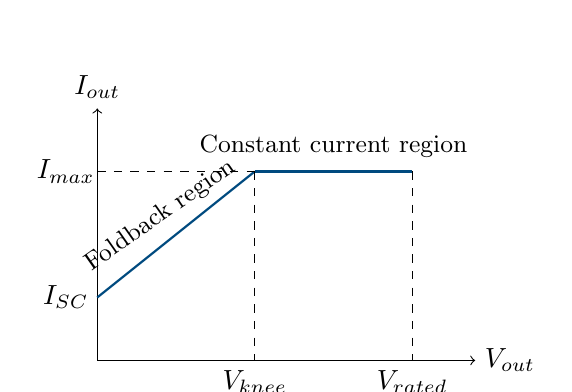
\begin{tikzpicture}[scale=0.8]
    % Axes
    \draw[->] (0,0) -- (6,0) node[right] {$V_{out}$};
    \draw[->] (0,0) -- (0,4) node[above] {$I_{out}$};
    
    % Curve
    \draw[thick,aoeblue] (5,3) -- (2.5,3);
    \draw[thick,aoeblue] (2.5,3) -- (0,1);
    
    % Labels
    \draw[dashed] (5,3) -- (5,0) node[below] {$V_{rated}$};
    \draw[dashed] (2.5,3) -- (2.5,0) node[below] {$V_{knee}$};
    \draw[dashed] (0,3) -- (2.5,3);
    \node at (-0.5,3) {$I_{max}$};
    \node at (-0.5,1) {$I_{SC}$};
    
    % Annotations
    \node at (3.75,3.4) {\small Constant current region};
    \node at (1,2.3) [rotate=35] {\small Foldback region};
\end{tikzpicture}
\caption{Foldback current limiting characteristic}
\label{fig:foldback}
\end{figure}

\subsection{Testing Procedures}

\subsubsection{Efficiency Measurement}

\begin{equation}
    \eta = \frac{P_{out}}{P_{in}} = \frac{V_{out} \times I_{out}}{V_{in} \times I_{in}} \times 100\%
\end{equation}

Measure at multiple load levels and output voltage settings.

\subsubsection{Transient Response Testing}

\begin{enumerate}[leftmargin=*]
    \item Apply a step load change (e.g., 10\% to 90\% of rated current)
    \item Capture output voltage on oscilloscope
    \item Measure: voltage dip/spike magnitude, recovery time
\end{enumerate}

\subsubsection{Protection Testing}

\begin{enumerate}[leftmargin=*]
    \item \textbf{Current Limit:} Gradually increase load until limiting engages
    \item \textbf{Short Circuit:} Apply brief short and verify safe behavior
    \item \textbf{Thermal:} Operate at high power and verify thermal shutdown (if implemented)
\end{enumerate}

\begin{deliverablebox}
\textbf{Phase 3 Deliverables:}
\begin{itemize}[leftmargin=*]
    \item Complete schematic with component values and thermal calculations
    \item Bill of materials with cost breakdown
    \item Efficiency measurements at various load and output voltage conditions
    \item Line and load regulation measurements
    \item Ripple waveforms at each output under load
    \item Transient response oscilloscope captures
    \item Protection testing documentation with photographs
    \item Thermal measurements at maximum load conditions
\end{itemize}
\end{deliverablebox}

\section{Phase 3 Checklist}

Before proceeding to Phase 4, verify:

\begin{itemize}
    \item[$\square$] All specified output rails functional and within tolerance
    \item[$\square$] Protection features tested and documented
    \item[$\square$] Efficiency measured and optimized where possible
    \item[$\square$] Thermal design adequate for sustained operation
    \item[$\square$] Documentation complete with test data and photographs
\end{itemize}

\clearpage

% ============================================================================
% PHASE 4: DIGITAL LOGIC & MIXED-SIGNAL
% ============================================================================
\chapter{Digital Logic, Interfaces, and Mixed-Signal Integration}
\label{ch:phase4}

\duration{4--5 weeks} \hfill \difficulty{Intermediate}

\vspace{0.5cm}

\begin{aoeref}
\textbf{Primary Reading:}
\begin{itemize}[leftmargin=*,nosep]
    \item Chapter 10: Digital Logic (10.1--10.8)
    \item Chapter 11: Programmable Logic Devices (11.1--11.4)
    \item Chapter 12: Logic Interfacing (12.1--12.8)
    \item Chapter 13: Digital Meets Analog (13.1--13.9)
\end{itemize}

\textbf{Supplementary from \xchapters:}
\begin{itemize}[leftmargin=*,nosep]
    \item Chapter 10x: Logic Pathology
    \item Chapter 13x: ADC and DAC Advanced Topics
\end{itemize}
\end{aoeref}

\vspace{0.5cm}

This phase bridges the analog and digital worlds. You will learn how to interface microcontrollers with analog circuits, convert signals between domains, and manage the unique challenges of mixed-signal systems.

\section{Phase Overview and Goals}

Modern instruments combine analog signal conditioning with digital processing, control, and communication. Success requires understanding both domains and their interaction---particularly how digital noise couples into sensitive analog circuits.

\begin{learningobjectives}
By the end of this phase, you will be able to:
\begin{enumerate}[leftmargin=*]
    \item Interface logic families (CMOS, LVTTL, etc.) with appropriate level shifting
    \item Design robust digital interfaces with proper termination and protection
    \item Select and interface ADCs and DACs for specified resolution and speed
    \item Partition mixed-signal PCB layouts to minimize noise coupling
    \item Implement basic microcontroller interfaces for measurement and control
    \item Debug timing, metastability, and signal integrity issues
    \item Apply decoupling and filtering strategies for mixed-signal systems
\end{enumerate}
\end{learningobjectives}

\section{Logic Families and Interfacing}

\subsection{Common Logic Families}

\begin{table}[H]
\centering
\caption{Logic Family Characteristics}
\label{tab:logic_families}
\begin{tabularx}{\textwidth}{@{}lXXXX@{}}
\toprule
\textbf{Family} & \textbf{Supply} & \textbf{$V_{OH}$ (min)} & \textbf{$V_{OL}$ (max)} & \textbf{Notes} \\
\midrule
5V CMOS (HC) & \SI{5}{\volt} & \SI{4.4}{\volt} & \SI{0.5}{\volt} & Standard 5V logic \\
3.3V LVCMOS & \SI{3.3}{\volt} & \SI{2.9}{\volt} & \SI{0.4}{\volt} & Common for modern MCUs \\
LVTTL & \SI{3.3}{\volt} & \SI{2.4}{\volt} & \SI{0.4}{\volt} & TTL-compatible thresholds \\
1.8V LVCMOS & \SI{1.8}{\volt} & \SI{1.45}{\volt} & \SI{0.35}{\volt} & Low-power digital \\
\bottomrule
\end{tabularx}
\end{table}

\subsection{Level Shifting}

When interfacing between different logic levels:

\begin{itemize}[leftmargin=*]
    \item \textbf{5V to 3.3V:} Resistor divider (simple, slow) or dedicated level shifter (TXB0108, etc.)
    \item \textbf{3.3V to 5V:} Many 5V CMOS inputs accept 3.3V directly; otherwise use buffers or MOSFETs
    \item \textbf{Bidirectional:} Dedicated bidirectional level shifters or MOSFET-based circuits
\end{itemize}

\section{ADC and DAC Fundamentals}

\subsection{ADC Selection Criteria}

\begin{table}[H]
\centering
\caption{ADC Architecture Comparison}
\label{tab:adc_comparison}
\begin{tabularx}{\textwidth}{@{}lXXX@{}}
\toprule
\textbf{Architecture} & \textbf{Speed} & \textbf{Resolution} & \textbf{Best For} \\
\midrule
Flash & $>$ \SI{100}{\mega\sample/\second} & 6--8 bits & Video, high-speed sampling \\
SAR & \SI{1}{\kilo\sample/\second}--\SI{10}{\mega\sample/\second} & 10--18 bits & General-purpose, MCU-integrated \\
Sigma-Delta & \SI{10}{\sample/\second}--\SI{1}{\mega\sample/\second} & 16--24 bits & Precision, low-frequency \\
Pipelined & \SI{10}{\mega\sample/\second}--\SI{500}{\mega\sample/\second} & 8--14 bits & High-speed with moderate resolution \\
\bottomrule
\end{tabularx}
\end{table}

\subsection{Effective Number of Bits (ENOB)}

Real ADC performance is limited by noise and distortion:

\begin{equation}
    ENOB = \frac{SINAD - 1.76}{6.02}
\end{equation}

where SINAD is signal-to-noise-and-distortion ratio in dB.

A 16-bit ADC may have an ENOB of only 12--14 bits in a practical system.

\section{Core Project: Mixed-Signal Measurement \& Control Unit}

\begin{projectbox}
\textbf{Project Title:} Digital Instrument Controller

\textbf{Objective:} Build a microcontroller-based system that interfaces with analog circuits from previous phases, demonstrating proper mixed-signal design practices.

\textbf{Time Estimate:} 15--20 hours
\end{projectbox}

\subsection{System Requirements}

\begin{itemize}[leftmargin=*]
    \item Read at least one analog signal (from precision AFE or power supply feedback)
    \item Provide a user interface (buttons/encoder for input, display for output)
    \item Control at least one output (relay, MOSFET, or DAC-driven setpoint)
    \item Demonstrate clean partitioning of analog and digital domains
\end{itemize}

\subsection{Microcontroller Selection}

For this project, select a microcontroller platform based on your experience:

\begin{itemize}[leftmargin=*]
    \item \textbf{Beginner:} Arduino (ATmega328P, ESP32)
    \item \textbf{Intermediate:} STM32 (Nucleo boards), Teensy
    \item \textbf{Advanced:} Custom design with bare MCU or FPGA + soft-core
\end{itemize}

The focus is on the electronics interfacing, not firmware complexity.

\subsection{Interface Design Requirements}

\subsubsection{Analog Input Interface}

\begin{itemize}[leftmargin=*]
    \item Input protection (clamping diodes, series resistors)
    \item Anti-alias filtering ($f_c < f_s/2$)
    \item Voltage scaling to match ADC input range
    \item Isolation from digital noise (physical separation, filtering)
\end{itemize}

\subsubsection{User Interface}

\begin{itemize}[leftmargin=*]
    \item Debounced pushbuttons (hardware RC or software debouncing)
    \item Rotary encoder with proper pull-ups and filtering
    \item Display interface (I2C OLED, SPI LCD, or parallel character LCD)
\end{itemize}

\subsubsection{Output Control}

\begin{itemize}[leftmargin=*]
    \item Relay driver with flyback protection
    \item MOSFET switch with gate drive considerations
    \item Optoisolator for ground isolation if needed
\end{itemize}

\subsection{PCB Layout Guidelines}

\begin{tipbox}
Mixed-signal layout rules:
\begin{enumerate}[leftmargin=*,nosep]
    \item Separate analog and digital ground planes; connect at a single point near the ADC
    \item Route analog signals away from digital signals, especially clocks
    \item Place decoupling capacitors as close as possible to IC power pins
    \item Use ground plane(s) under all signal traces
    \item Keep analog components on opposite side of board from digital
    \item Use star power distribution from the main filter capacitors
\end{enumerate}
\end{tipbox}

\begin{deliverablebox}
\textbf{Phase 4 Deliverables:}
\begin{itemize}[leftmargin=*]
    \item Complete schematic showing analog, digital, and power partitioning
    \item PCB layout (if fabricated) or annotated breadboard photos
    \item Timing diagrams for key interfaces (hand-drawn acceptable)
    \item Noise measurement: analog signal with digital circuitry running vs. stopped
    \item Demonstration of complete system operation
    \item Written ``EMI/noise lessons learned'' document
\end{itemize}
\end{deliverablebox}

\section{Phase 4 Checklist}

Before proceeding to Phase 5, verify:

\begin{itemize}
    \item[$\square$] Microcontroller interface functional with analog front-end
    \item[$\square$] User interface (display, buttons) operating correctly
    \item[$\square$] Output control (relay/MOSFET) functioning as designed
    \item[$\square$] Noise coupling documented and minimized
    \item[$\square$] Documentation complete with timing analysis
\end{itemize}

\clearpage

% ============================================================================
% PHASE 5: HIGH-SPEED & RF-LITE
% ============================================================================
\chapter{High-Speed, RF-Lite, and Signal Integrity}
\label{ch:phase5}

\duration{4--6 weeks (Optional, Advanced)} \hfill \difficulty{Advanced}

\vspace{0.5cm}

\begin{aoeref}
\textbf{Primary Reading:}
\begin{itemize}[leftmargin=*,nosep]
    \item Appendix H: Transmission Lines
    \item Chapter 7: Oscillators (7.1--7.3)
    \item Chapter 13: Digital Meets Analog (high-speed sections)
\end{itemize}

\textbf{Supplementary from \xchapters:}
\begin{itemize}[leftmargin=*,nosep]
    \item Chapter 1x: Real-World Passive Components (parasitics at high frequency)
    \item Chapter 4x: High-Speed Amplifiers
\end{itemize}
\end{aoeref}

\vspace{0.5cm}

This optional phase pushes into territory where wires become transmission lines, capacitors become inductors, and your intuition from low-frequency work may mislead you.

\section{Phase Overview and Goals}

\begin{learningobjectives}
By the end of this phase, you will be able to:
\begin{enumerate}[leftmargin=*]
    \item Identify when transmission line effects become significant
    \item Design proper termination for various signal types
    \item Recognize and diagnose reflections, ringing, and crosstalk
    \item Select and apply high-speed op-amps correctly
    \item Implement basic clock generation and distribution
    \item Use time-domain reflectometry concepts for diagnosis
\end{enumerate}
\end{learningobjectives}

\section{When Does High-Speed Matter?}

The rule of thumb: treat a trace as a transmission line when:

\begin{equation}
    l > \frac{\lambda}{10} = \frac{v_p}{10 \times f}
\end{equation}

where $l$ is trace length, $\lambda$ is wavelength, $v_p$ is propagation velocity ($\approx$ 0.5c for typical PCB), and $f$ is the highest significant frequency.

For edge rate considerations, use the rise/fall time:

\begin{equation}
    f_{knee} \approx \frac{0.35}{t_r}
\end{equation}

\textbf{Example:} A signal with \SI{1}{\nano\second} rise time has frequency content up to approximately \SI{350}{\mega\hertz}. At this frequency, any trace longer than about \SI{4}{\centi\meter} is a transmission line.

\section{Core Project: High-Speed Buffer / Line Driver}

\begin{projectbox}
\textbf{Project Title:} 50$\Omega$ Line Driver with Transmission Line Experiments

\textbf{Objective:} Design a fast buffer capable of driving a matched \SI{50}{\ohm} load through coaxial cable, and experimentally observe transmission line effects.

\textbf{Time Estimate:} 10--15 hours
\end{projectbox}

\subsection{Specifications}

\begin{itemize}[leftmargin=*]
    \item Output: \SI{50}{\ohm} matched, capable of $\pm$\SI{2}{\volt} into \SI{50}{\ohm}
    \item Bandwidth: DC to \SI{50}{\mega\hertz} (minimum)
    \item Rise time: $<$ \SI{5}{\nano\second}
    \item Square wave: Clean edges at \SI{10}{\mega\hertz}
\end{itemize}

\subsection{Experiments}

\subsubsection{Experiment A: Termination Effects}

Using a length of coaxial cable (e.g., \SI{3}{\meter} of RG-58):

\begin{enumerate}[leftmargin=*]
    \item Measure with proper \SI{50}{\ohm} termination
    \item Measure with open circuit (no termination)
    \item Measure with short circuit
    \item Measure with \SI{100}{\ohm} and \SI{25}{\ohm} (mismatch cases)
\end{enumerate}

Document the reflections, overshoot, and ringing in each case.

\subsubsection{Experiment B: Cable Length Effects}

With proper termination, compare:
\begin{enumerate}[leftmargin=*]
    \item \SI{0.5}{\meter} cable
    \item \SI{3}{\meter} cable
    \item \SI{10}{\meter} cable
\end{enumerate}

Observe propagation delay and any attenuation.

\begin{deliverablebox}
\textbf{Phase 5 Deliverables:}
\begin{itemize}[leftmargin=*]
    \item Schematic of high-speed buffer with layout considerations documented
    \item Oscilloscope captures showing reflections under various termination conditions
    \item Annotated waveforms correlating observations with transmission line theory
    \item Written summary translating AoE theory into observed phenomena
\end{itemize}
\end{deliverablebox}

\clearpage

% ============================================================================
% PHASE 6: CAPSTONE
% ============================================================================
\chapter{Capstone: Integrated Instrument or System}
\label{ch:phase6}

\duration{6--8+ weeks} \hfill \difficulty{Advanced}

\vspace{0.5cm}

The capstone project integrates knowledge and skills from all previous phases into a single, substantial piece of equipment worthy of a permanent place on your bench.

\section{Phase Overview and Goals}

The capstone is intentionally open-ended. You will define requirements, make design trade-offs, and execute a complete engineering project from concept to characterized prototype.

\begin{learningobjectives}
By the end of this phase, you will have:
\begin{enumerate}[leftmargin=*]
    \item Defined and documented a complete system specification
    \item Made and justified architectural decisions
    \item Integrated analog, digital, and power subsystems
    \item Characterized performance against specifications
    \item Identified limitations and potential improvements
    \item Produced professional-quality documentation
\end{enumerate}
\end{learningobjectives}

\section{Capstone Project Options}

Choose one of the following, or propose your own with instructor approval:

\subsection{Option A: Modular Data Acquisition System}

A multi-channel measurement system with:
\begin{itemize}[leftmargin=*]
    \item 4+ analog input channels with configurable gain and filtering
    \item 16-bit or better resolution
    \item Software-configurable sample rate (\SI{1}{\sample/\second} to \SI{10}{\kilo\sample/\second})
    \item Data logging to SD card or USB
    \item Display of real-time measurements
    \item Alarm thresholds with audible/visual indicators
\end{itemize}

\subsection{Option B: Precision Bench Instrument}

A high-accuracy voltmeter or current meter featuring:
\begin{itemize}[leftmargin=*]
    \item 5.5-digit resolution (minimum)
    \item Multiple ranges with auto-ranging capability
    \item True RMS AC measurement
    \item Data hold and min/max capture
    \item RS-232 or USB data output
\end{itemize}

\subsection{Option C: Smart Power Platform}

An advanced bench power supply with:
\begin{itemize}[leftmargin=*]
    \item Digital control of voltage and current limits
    \item Real-time monitoring of output power
    \item Sequencing capability for multi-rail applications
    \item Battery charging profiles
    \item USB interface for computer control
    \item Extensive protection with fault logging
\end{itemize}

\section{Capstone Requirements}

Regardless of project choice, you must deliver:

\subsection{System Architecture Document}

\begin{itemize}[leftmargin=*]
    \item Block diagram showing all subsystems and their interconnections
    \item Justification for key design choices with AoE references
    \item Trade-off analyses (e.g., linear vs. switching, resolution vs. speed)
    \item Risk assessment and mitigation strategies
\end{itemize}

\subsection{Complete Schematics and Layout}

\begin{itemize}[leftmargin=*]
    \item Professional-quality schematics with component values
    \item Clear labeling of functional blocks
    \item Layout showing analog/digital partitioning
    \item Grounding, shielding, and decoupling strategies annotated
\end{itemize}

\subsection{Test and Characterization Plan}

\begin{itemize}[leftmargin=*]
    \item Definition of key performance metrics
    \item Test procedures for each metric
    \item Required equipment and calibration references
    \item Pass/fail criteria based on specifications
\end{itemize}

\subsection{Test Results and Analysis}

\begin{itemize}[leftmargin=*]
    \item Complete test data in tabular and graphical form
    \item Comparison of measured vs. specified performance
    \item Analysis of any discrepancies
    \item Recommendations for improvement
\end{itemize}

\subsection{Reflection Document}

\begin{itemize}[leftmargin=*]
    \item What AoE concepts proved most valuable
    \item What only became clear through building and measuring
    \item Biggest challenges and how you overcame them
    \item What you would do differently in a second iteration
\end{itemize}

\begin{deliverablebox}
\textbf{Capstone Deliverables Summary:}
\begin{itemize}[leftmargin=*]
    \item System Architecture Document (5--10 pages)
    \item Complete Schematic Package (all sheets, BOM)
    \item Layout Files or Annotated Assembly Photographs
    \item Test and Characterization Report (10--20 pages)
    \item Working Prototype (demonstrated)
    \item Reflection Document (2--3 pages)
    \item 15-minute Presentation (optional, for formal courses)
\end{itemize}
\end{deliverablebox}

\clearpage

% ============================================================================
% APPENDICES
% ============================================================================
\appendix

\chapter{How to Use \aoe{} Along the Way}
\label{app:using_aoe}

This appendix provides structured guidance for integrating \aoe{} reading with hands-on project work.

\section{Pre-Reading Strategy}

Before each phase:

\begin{enumerate}[leftmargin=*]
    \item Skim the relevant AoE sections listed in the phase introduction
    \item Write down 3--5 rules-of-thumb or ``red flags'' you'll watch for
    \item Note any unfamiliar terms or concepts for deeper study
    \item Review the figures and schematics---they often convey more than the text
\end{enumerate}

\section{Design Bookmarking}

As you design your circuits:

\begin{enumerate}[leftmargin=*]
    \item Annotate schematics with AoE references:
    \begin{itemize}
        \item ``Compensation network inspired by AoE §4.9.2''
        \item ``Snubber per AoE's rectifier surge suppression guidance''
    \end{itemize}
    \item Record your predictions based on AoE rules-of-thumb
    \item Note any deviations from AoE's recommended approaches and why
\end{enumerate}

\section{Post-Mortem Reading}

After measuring your circuits:

\begin{enumerate}[leftmargin=*]
    \item Return to AoE and compare your issues with their troubleshooting advice
    \item Use their oscilloscope screenshots as reference for diagnosing odd behavior
    \item Update your notes with what you learned from the discrepancies
    \item Consider: Would following AoE more closely have avoided the problem?
\end{enumerate}

\chapter{Equipment Recommendations}
\label{app:equipment}

\section{Budget-Conscious Setup}

For students or hobbyists on a budget, these minimum specifications will suffice:

\begin{itemize}[leftmargin=*]
    \item \textbf{Oscilloscope:} Rigol DS1054Z or similar (4-channel, \SI{50}{\mega\hertz}, upgradeable)
    \item \textbf{Function Generator:} FY6900 or similar DDS generator
    \item \textbf{Power Supply:} Basic dual-rail linear supply or repurposed ATX supply
    \item \textbf{Multimeter:} Any 4.5-digit handheld with true RMS
    \item \textbf{Soldering:} Temperature-controlled station (Hakko FX-888D or similar)
\end{itemize}

\section{Professional Setup}

For serious laboratories or teaching environments:

\begin{itemize}[leftmargin=*]
    \item \textbf{Oscilloscope:} \SI{200}{\mega\hertz}+ bandwidth, \SI{1}{\giga\sample/\second}+, MSO capability
    \item \textbf{Function Generator:} \SI{25}{\mega\hertz}+ arbitrary waveform generator
    \item \textbf{Power Supply:} Programmable with sequencing and data logging
    \item \textbf{Multimeter:} 6.5-digit bench multimeter with GPIB/USB
    \item \textbf{Additional:} Spectrum analyzer, LCR meter, curve tracer
\end{itemize}

\chapter{Component Sources}
\label{app:components}

\section{Major Distributors}

\begin{itemize}[leftmargin=*]
    \item \textbf{Digi-Key} (digikey.com): Comprehensive selection, excellent parametric search
    \item \textbf{Mouser} (mouser.com): Similar to Digi-Key, strong on passives
    \item \textbf{Newark/Farnell} (newark.com): Good for industrial and European parts
    \item \textbf{Arrow} (arrow.com): Competitive pricing on volume orders
\end{itemize}

\section{Budget Options}

\begin{itemize}[leftmargin=*]
    \item \textbf{LCSC} (lcsc.com): Low-cost components from China, good for basic parts
    \item \textbf{AliExpress}: Inexpensive component kits and modules (verify authenticity)
    \item \textbf{eBay}: Useful for vintage or hard-to-find parts (beware counterfeits)
\end{itemize}

\section{Specialty Suppliers}

\begin{itemize}[leftmargin=*]
    \item \textbf{Texas Instruments} (ti.com): Free samples for students
    \item \textbf{Analog Devices} (analog.com): Sample programs available
    \item \textbf{Mini-Circuits} (minicircuits.com): RF components and test equipment
\end{itemize}

% ============================================================================
% BACK MATTER
% ============================================================================
\backmatter

\chapter*{Final Notes}

This curriculum provides a framework, not a prescription. Adapt the projects to your interests, available equipment, and learning goals. The most important thing is to build, measure, and iterate.

\aoe{} is a dense text, and you will not absorb everything on first reading. That's intentional. Return to it throughout your electronics career, and you will find new insights each time.

The electronics laboratory is a place of continuous learning. Every circuit that doesn't work as expected is an opportunity to deepen your understanding. Embrace the debugging process---it's where real expertise is built.

\vspace{2cm}

\begin{center}
\textit{Build well. Measure carefully. Learn continuously.}
\end{center}

\end{document}
